% Created 2024-09-16 Mon 21:35
% Intended LaTeX compiler: pdflatex
\documentclass[aspectratio=169,xcolor={dvipsnames,svgnames}]{beamer}
\usepackage[utf8x]{inputenc}
\usepackage[T1]{fontenc}
\usepackage{graphicx}
\usepackage{longtable}
\usepackage{wrapfig}
\usepackage{rotating}
\usepackage[normalem]{ulem}
\usepackage{amsmath}
\usepackage{amssymb}
\usepackage{capt-of}
\usepackage{hyperref}
\usepackage{minted}
\usepackage{libertine}
\usepackage[normalem]{ulem}
\usepackage{varwidth}
\usepackage[Export]{adjustbox}
%\usepackage{enumitem}
\usepackage[linesnumbered,ruled,vlined]{algorithm2e}
\graphicspath{ {./images/} {./org-download-images/} }
\usepackage[date=year,%
backend=biber,%
style=alphabetic,%
maxnames=5,%
minnames=3,%
maxalphanames=4,%
minalphanames=3,%
backref=true,%
doi=false,%
isbn=false,%
url=false,%
eprint=false]{biblatex}
\DefineBibliographyStrings{english}{%
backrefpage  = {\lowercase{s}ee p.}, % for single page number
backrefpages = {\lowercase{s}ee pp.} % for multiple page numbers
}
\addbibresource{/home/bvraghav/bibliography.bib}
%% Math typesetting
%% --------------------------------
\usepackage{amsmath}
\usepackage{amssymb}
\usepackage{amsfonts}
\usepackage{bbold}
% Operators with limit-style sub and superscript
\DeclareMathOperator*{\E}{\mathbb{E}}
\hypersetup{%
colorlinks=true,%
allcolors=magenta,%
%linkbordercolor = {white},%
%<your other options...>,
}
\usetheme{boxes}
\usecolortheme{crane}
\usefonttheme{serif}
\useinnertheme{rectangles}
\useoutertheme{}
\date{\textit{[2024-07-15 Mon]}}
\title{Overview}
\subtitle{ucs749: speech processing and synthesis}
\author{%
%\noindent{} \\[2em]
\normalsize Raghav B. Venkataramaiyer
}
\institute{%
CSED TIET Patiala India.
}
\date{\scriptsize \today}
\setbeamercolor{alerted text}{fg=red!80!black}
%% Setup outline at begin section
%% -------------------------------------------------------
\AtBeginSection[]               % Section
{
\begin{frame}{outline}
\tableofcontents[currentsection,hideallsubsections]
\end{frame}
}
\AtBeginSubsection[]            % SubSection
{
\begin{frame}{outline}
\tableofcontents[currentsection,currentsubsection,subsectionstyle=show/shaded/hide]
\end{frame}
}
\setbeamerfont{structure}{shape=\scshape,family=\sffamily}
\setbeamertemplate{section page}
{
\begin{centering}
\begin{beamercolorbox}[sep=12pt,center]{part title}
\usebeamerfont{section title}\insertsection\par
\end{beamercolorbox}
\end{centering}
}

\setbeamercovered{transparent}
\hypersetup{
 pdfauthor={Raghav B. Venkataramaiyer},
 pdftitle={Overview},
 pdfkeywords={},
 pdfsubject={},
 pdfcreator={Emacs 29.4 (Org mode 9.6.24)}, 
 pdflang={English}}
\begin{document}

\maketitle
\begin{frame}{Outline}
\tableofcontents
\end{frame}


\section{about}
\label{sec:org080330f}
\begin{frame}[label={sec:org1cf6eb7}]{course weightage}
\begin{center}
\begin{tabular}{rrrr}
L & T & P & Cr\\[0pt]
\hline
2 & 0 & 2 & 3\\[0pt]
\end{tabular}
\end{center}
\end{frame}

\begin{frame}[label={sec:orge77f31b}]{syllabus}
\href{ucs749-syllabus.pdf}{Link to Syllabus [PDF]​}
\end{frame}

\begin{frame}[label={sec:org0ce9054}]{academic calendar}
\begin{figure}[htbp]
\centering
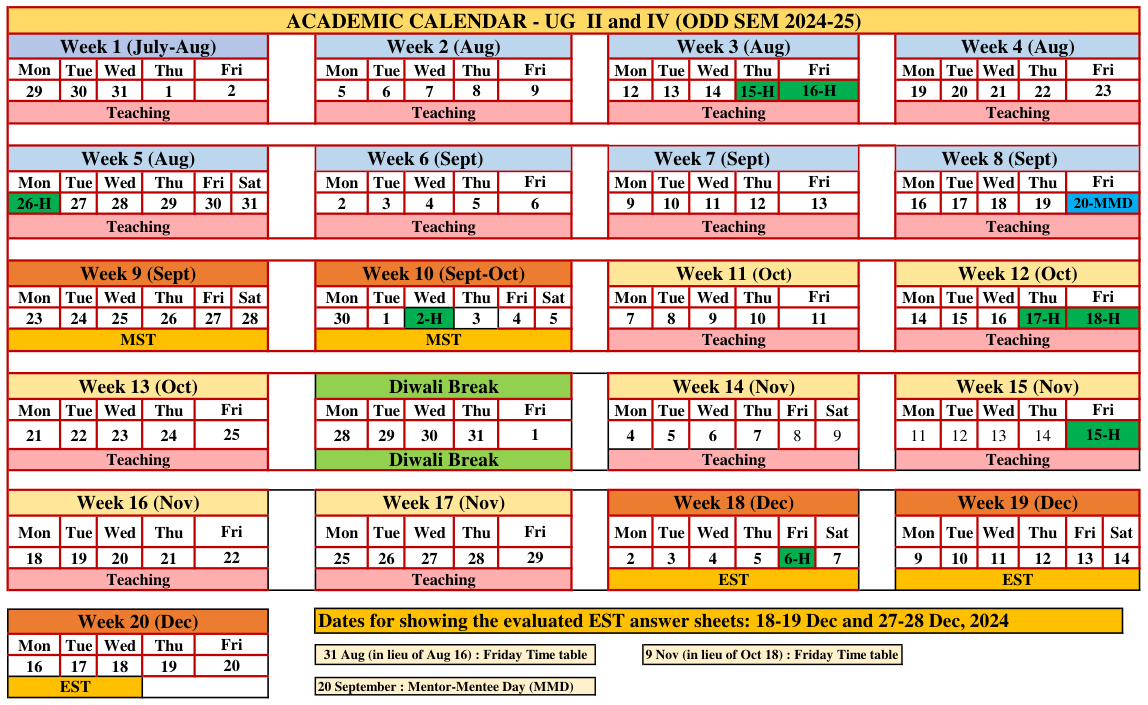
\includegraphics[width=.9\linewidth]{image/2024-07-15_22-56-44_screenshot.png}
\caption{Academic Calendar}
\end{figure}
\end{frame}

\begin{frame}[label={sec:orgd8325f1}]{num lectures}
\begin{center}
\begin{tabular}{lrrl}
 & W & L & P\\[0pt]
\hline
Prior to MST & 8 & 16 & 7/8\\[0pt]
MST -- Diwali & 3 & 6 & 2/3\\[0pt]
Diwali -- EST & 4 & 8 & 4\\[0pt]
\end{tabular}
\end{center}
\end{frame}

\section{evaluation}
\label{sec:org27d22e2}

\begin{frame}[label=evaluation-schedule]{evaluation schedule}
\begin{center}
\begin{tabular}{llr}
 & Date & MM\\[0pt]
\hline
MST & TBA & 30\\[0pt]
EST & TBA & 40\\[0pt]
Quiz 1 & \sout{12-Sep 05:30pm} & 5\\[0pt]
Quiz 2 & 21-Nov 05:30pm & 5\\[0pt]
Lab Eval 1 & \sout{9-Sep 13-Sep} & 10\\[0pt]
Lab Eval 2 & 18-Nov -- 22-Nov & 10\\[0pt]
\hline
 &  & 100\\[0pt]
\end{tabular}
\end{center}
\end{frame}

\begin{frame}[label={sec:about-lab-eval}]{about lab eval}
All exercise(s) shall be solved in (Colab) python
notebook(s), committed to Github using @thapar.edu
account.  Only a Github Repo link and commit id shall
be submit using the Google Form. Any attachments are
\alert{not} allowed.  \href{./about-lab-eval/}{[Read more\ldots{}]​}
\end{frame}

\section{topics}
\label{schedule-of-topics}
\subsection{Background}
\label{sec:org4d73964}
\begin{frame}[label={sec:org738baf7}]{pre-requisites}
\begin{enumerate}
\item \href{https://www.3blue1brown.com/topics/linear-algebra}{Linear Algebra}: Vector Spaces/ Linear Maps/
Singularity/ Matrix Decomposition/ Null
Space/ Span/ Markov Chains;
\item Probability and Statistics: Central Limit
Theorem/ Conditionals \& Marginals/ Bayes
Theorem/ Markov Assumption/ Stochastic
Process
\item Information Theory: Cross Entropy
\item Neural Network: Perceptron Model/ Hidden
Layers/ Convolution/ Activation/ Pooling/
Atrous/ Padding/ Backpropagationჲ
\item Optimisation: Stochastic Gradient Descent/
Momentum/ Dropout/ RMSProp/ Adam
\item Deep Learning: Sequential Model/ Residual Model/
Adversarial Model/ Attention Model/ Encoder-Decoder
Model
\end{enumerate}
\end{frame}

\begin{frame}[label=schedule-introduction]{introduction}
\begin{enumerate}
\item NLP: Lexeme/ Grapheme
\item Speech: Phoneme
\item Statistical Models: Noise/ Pattern/
Characterisation
\item Language Model: N-Grams/ TFIDF/ Word2Vec/ BERT
\item Speech Models: Wav2Vec/ HuBERT
\end{enumerate}
\end{frame}

\subsection{Recognition}
\label{sec:org9064009}

\begin{frame}[label=schedule-recognition]{automated speech recognition}
\begin{description}
\item[{Hidden Markov Model}] \href{https://web.stanford.edu/\~jurafsky/slp3/A.pdf}{PDF (Concise)}, More literature
from \href{https://www.google.com/search?hl=en\&q=hidden\%20markov\%20model\%20filetype\%3Apdf}{Google}, \href{https://duckduckgo.com/?q=hidden+markov+model+filetype\%3Apdf\&ia=web}{Duck,Duck,Go}; \href{https://scholar.google.com/scholar?q=A\%20tutorial\%20on\%20hidden\%20Markov\%20models\%20and\%20selected\%20applications\%20in\%20speech\%20recognition}{Rabiner’s Tutorial}.
\item[{Time Delay DNN (TDNN)}] \begin{itemize}
\item \href{./time-delay-networks/}{Time-delay Networks (TDNN)},
\item \href{./ctc/}{Connectionist Temporal Classification (CTC)},
\item \href{./jasper/}{Jasper},
\item \href{https://paperswithcode.com/paper/quartznet-deep-automatic-speech-recognition}{QuartzNet},
\item \href{https://paperswithcode.com/paper/citrinet-closing-the-gap-between-non}{Citrinet}
\end{itemize}
\item[{Speech Command Recognition}] MatchboxNet: \href{https://paperswithcode.com/paper/matchboxnet-1d-time-channel-separable-1}{[PwC]​}
\href{https://colab.research.google.com/github/tiet-ucs749/tiet-ucs749.github.io/blob/main/matchboxnet/Speech\_Commands.ipynb}{[Colab]​} (Implementation: \href{https://github.com/google-research/google-research/blob/master/kws\_streaming/models/ds\_tc\_resnet.py}{here} and \href{https://github.com/google-research/google-research/blob/master/kws\_streaming/models/xception.py}{here} uses \href{https://github.com/google-research/google-research/blob/master/kws\_streaming/models/xception.py\#L252-L266}{AvgPool
after blocks})
\end{description}
\end{frame}

\subsection{Synthesis}
\label{sec:orgb6dd743}
\begin{frame}[label=schedule-synthesis]{synthesis (text-to-speech; tts)}
\begin{description}
\item[{Spectrogram Generators}] \href{https://paperswithcode.com/paper/natural-tts-synthesis-by-conditioning-wavenet}{Tacotron2}, \href{https://paperswithcode.com/paper/glow-tts-a-generative-flow-for-text-to-speech}{GlowTTS}
\item[{Audio Generators}] \href{https://paperswithcode.com/paper/waveglow-a-flow-based-generative-network-for}{WaveGlow}, \href{https://cs.paperswithcode.com/paper/squeezewave-extremely-lightweight-vocoders}{SqueezeWave}
\end{description}
\end{frame}

\section{practicals}
\label{schedule-of-practicals}
\begin{frame}[label=lab-1]{lab 1: getting familiar with speech processing}
\begin{enumerate}
\item Getting familiar with the pipeline of Speech
Recognition: \\[0pt]
\href{https://pytorch.org/audio/stable/tutorials/speech\_recognition\_pipeline\_tutorial.html}{Speech Recognition with Wav2Vec2} (Pytorch)
\item Perform a simple command classification task with
a sequential model:
\begin{itemize}
\item (Tensorflow) \href{https://www.tensorflow.org/tutorials/audio/simple\_audio}{Simple Audio Recognition :Recognising
keywords}; or if you prefer
\item (Pytorch) \href{https://pytorch.org/tutorials/intermediate/speech\_command\_classification\_with\_torchaudio\_tutorial.html}{Speech Command Classification with M5}.
\end{itemize}
\end{enumerate}
\end{frame}

\begin{frame}[label=lab-2]{lab 2: hidden markov model}
Using MFCCs as features from this example: \\[0pt]
\href{https://colab.research.google.com/drive/1pkopM-0bSoxH1WDwq94bFSBxXpkHrjI3?usp=sharing}{MFCC Example [Colab]​} by \href{https://github.com/bvraghav}{Raghav B. Venkataramaiyer};\\[0pt]
along with the following dataset: \\[0pt]
\href{https://github.com/Jakobovski/free-spoken-digit-dataset}{Free Spoken Digit Dataset (10 digits x 6 speakers x 50
repeats) [Github]​}; \\[0pt]
and using hmmlearn as in this tutorial to fit the
model \\[0pt]
\href{https://hmmlearn.readthedocs.io/en/latest/tutorial.html}{HMM Learn [ReadTheDocs]​}

\begin{enumerate}
\item Compute the probability of occurrence of a given
sequence, say \(\{3,2,5,4,0\}\). (Encode the Forward
Algorithm)
\item Predict the most likely sequence, given an audio
sequence. (Encode the Viterbi algorithm)
\end{enumerate}
\end{frame}

\begin{frame}[label={sec:orgdeeff8f}]{lab 2: hidden markov model (contd…)}
\begin{description}
\item[{Theory}] \href{https://web.stanford.edu/\~jurafsky/slp3/A.pdf}{PDF (Concise)}, More literature from \href{https://www.google.com/search?hl=en\&q=hidden\%20markov\%20model\%20filetype\%3Apdf}{Google},
\href{https://duckduckgo.com/?q=hidden+markov+model+filetype\%3Apdf\&ia=web}{Duck,Duck,Go}; \href{https://scholar.google.com/scholar?q=A\%20tutorial\%20on\%20hidden\%20Markov\%20models\%20and\%20selected\%20applications\%20in\%20speech\%20recognition}{Rabiner's Tutorial}.
\item[{More Datasets}] \href{https://code.google.com/archive/p/hmm-speech-recognition/downloads}{hmm-speech-recognition [Google Code]​}
\item[{More Feature Descriptors}] \href{https://en.wikipedia.org/wiki/Cepstral\_mean\_and\_variance\_normalization}{CMVN}, \href{http://people.csail.mit.edu/sshum/talks/ivector\_tutorial\_interspeech\_27Aug2011.pdf}{i-vectors}
\item[{See Also}] \begin{itemize}
\item \href{https://colab.research.google.com/github/bambschool/BAMB2023/blob/main/6-latent\_variable\_models/hidden-markov-models.ipynb}{HMM Tutorial [Colab]​} by \href{https://github.com/bambschool/BAMB2023}{BAMB School 2023}
\item \href{https://colab.research.google.com/github/facebookresearch/beanmachine/blob/main/tutorials/Hidden\_Markov\_model.ipynb\#scrollTo=vwxlljQwXOxg}{Bean-Machine based Tutorial [Colab]​}
\item \href{https://medium.com/@natsunoyuki/hidden-markov-models-with-python-c026f778dfa7}{HMM Predicting Gold Prices [Medium]​}
\item \href{https://colab.research.google.com/github/kastnerkyle/kastnerkyle.github.io/blob/master/posts/single-speaker-word-recognition-with-hidden-markov-models/single-speaker-word-recognition-with-hidden-markov-models.ipynb}{Single Speaker Word Recognition with HMM [Colab]​}
\item \href{https://colab.research.google.com/drive/1aFgzrUv3udM\_gNJNUoLaHIm78QHtxdIz?usp=sharing}{ASR using HMM from scratch [Colab]​}
\end{itemize}
\end{description}
\end{frame}

\begin{frame}[label=lab-3,fragile]{lab 3: asr in english}
 \href{https://colab.research.google.com/github/NVIDIA/NeMo/blob/stable/tutorials/asr/ASR\_with\_NeMo.ipynb}{ASR with NeMo (Colab)}

Additional references:
\begin{itemize}
\item \href{https://nvidia.github.io/apex/amp.html\#opt-levels}{\texttt{amp\_level}"O1"= : the argument used in
\texttt{PytorchLightning.Trainer} instance};
\item But \href{https://github.com/Lightning-AI/pytorch-lightning/pull/16039}{Apex deprecated out of PL} v2.0;
\end{itemize}

For Starters : \\[0pt]
\href{https://docs.nvidia.com/nemo-framework/user-guide/latest/nemotoolkit/starthere/intro.html\#quick-start-guide}{NeMo Installation and Getting Started Guide with
Citrinet ASR Evaluation}
\end{frame}

\begin{frame}[label=lab-4]{lab 4: asr in indic language}
Use the method from Lab 3, but use \href{https://github.com/AI4Bharat/vistaar}{Indic Dataset}.
\end{frame}

\begin{frame}[label=lab-5]{lab 5: speech commands}
\href{https://colab.research.google.com/github/NVIDIA/NeMo/blob/stable/tutorials/asr/Speech\_Commands.ipynb}{Speech Command Recognition with MatchboxNet}
\end{frame}

\begin{frame}[label=lab-6]{lab 6: tts with tacotron 2}
\href{https://colab.research.google.com/github/NVIDIA/NeMo/blob/stable/tutorials/tts/Tacotron2\_Training.ipynb}{Training with Tacotron 2}
\end{frame}

\begin{frame}[label=lab-7]{lab 7: tts in indic language}
Use the method from Lab 6, but along with \href{https://github.com/AI4Bharat/Indic-TTS}{Indic Dataset
for TTS}.
\end{frame}

\section{resources}
\label{resources}
\begin{frame}[label={sec:org3158637}]{speech}
\begin{enumerate}
\item \href{https://github.com/wenet-e2e/speech-synthesis-paper}{Directory Listing of SoTA}
\item \href{https://github.com/zzw922cn/awesome-speech-recognition-speech-synthesis-papers}{Another Directory Listing of SoTA}
\item \href{https://arxiv.org/abs/1904.03288}{Jasper (2019)}
\item \href{https://arxiv.org/abs/1910.10261}{QuartzNet (2019)}
\item \href{https://arxiv.org/abs/2104.01721}{Citrinet (2021)}
\item \href{https://docs.nvidia.com/nemo-framework/user-guide/latest/nemotoolkit/asr/intro.html}{NVidia NeMo Framework}
\item \href{https://docs.nvidia.com/nemo-framework/user-guide/latest/nemotoolkit/tts/intro.html}{Speech Synthesis Model Zoo (NeMo)}
\item \href{https://medium.com/analytics-vidhya/understanding-the-mel-spectrogram-fca2afa2ce53}{Mel Spectrogram}
\end{enumerate}
\end{frame}

\begin{frame}[label={sec:orgbcd2da4}]{linear algebra}
\begin{enumerate}
\item \href{https://www.3blue1brown.com/topics/linear-algebra}{3B1B}
\item \href{https://ocw.mit.edu/courses/18-06-linear-algebra-spring-2010/}{Gilbert Strang}
\end{enumerate}
\end{frame}

\begin{frame}[label={sec:org1f00d65}]{probability and statistics}
\begin{enumerate}
\item Bertsekas \& Tsitsiklis: \href{https://ocw.mit.edu/courses/res-6-012-introduction-to-probability-spring-2018/}{Introduction To
Probability}; \href{https://ocw.mit.edu/courses/6-041sc-probabilistic-systems-analysis-and-applied-probability-fall-2013/}{Probabilistic Systems Analysis And
Applied Probability}
\item \href{https://www.3blue1brown.com/topics/probability}{3B1B}
\end{enumerate}
\end{frame}

\begin{frame}[label={sec:orge957e03}]{neural network concepts}
\begin{enumerate}
\item \href{https://www.coursera.org/specializations/deep-learning}{Andrew Ng on Coursera}
\item \href{https://www.youtube.com/playlist?list=PLkt2uSq6rBVctENoVBg1TpCC7OQi31AlC}{Andrej Karpathy on Youtube}; also on \href{https://cs231n.stanford.edu/2016/}{Stanford}
\end{enumerate}
\end{frame}

\begin{frame}[label={sec:orgb2cbd14}]{information theory \& learning}
\begin{enumerate}
\item \href{https://www.inference.org.uk/itila/}{David McKay}
\end{enumerate}
\end{frame}

\begin{frame}[label={sec:org991702d}]{datasets}
\begin{enumerate}
\item \href{https://pytorch.org/audio/stable/datasets.html}{Torch Audio (Pytorch)}
\item \href{https://www.tensorflow.org/datasets/catalog/overview\#speech}{Speech \& Speech Recognition Datasets (Tensorflow)}
\item \href{https://docs.nvidia.com/nemo-framework/user-guide/latest/nemotoolkit/asr/datasets.html}{ASR Datasets (NeMo)}
\item \href{https://docs.nvidia.com/nemo-framework/user-guide/latest/nemotoolkit/asr/speech\_classification/datasets.html}{Speech Classification Datasets (NeMo)}
\item \href{https://github.com/lhotse-speech/lhotse}{Lhotse Speech} and \href{https://docs.nvidia.com/nemo-framework/user-guide/latest/nemotoolkit/asr/datasets.html\#lhotse-dataloading}{its use with NeMo}
\item \href{https://docs.nvidia.com/nemo-framework/user-guide/latest/nemotoolkit/asr/speaker\_recognition/datasets.html}{Speaker Recognition Datasets (NeMo)}
\item \href{https://docs.nvidia.com/nemo-framework/user-guide/latest/nemotoolkit/tts/datasets.html\#public-tts-datasets}{Public TTS Datasets (NeMo)}
\item \href{https://github.com/AI4Bharat/vistaar}{Indic ASR Dataset}
\item \href{https://github.com/AI4Bharat/Indic-TTS}{Indic Dataset for TTS}
\end{enumerate}
\end{frame}

\begin{frame}[label={sec:orgb4fd9a0}]{code}
\begin{enumerate}
\item \href{https://github.com/NVIDIA/OpenSeq2Seq}{OpenSeq2Seq}
\item \href{https://github.com/AI4Bharat/Indic-TTS}{AI4Bharat}
\item \href{https://github.com/NVIDIA/NeMo/tree/stable/tutorials/}{NeMo Tutorials}
\end{enumerate}
\end{frame}

\section{introduction}
\label{schedule-introduction}
\subsection{Parallels b/w NLP and Speech}
\label{sec:orgd34f472}
\begin{frame}[label={sec:org0cea720}]{nlp}
\begin{description}
\item[{Natural Language Processing}] Lexeme/ Grapheme
\item[{Language Models}] \begin{description}
\item[{Statistical Models}] N-Grams/ TFIDF
\item[{Recently}] Word2Vec/ BERT etc.
\end{description}
\end{description}
\end{frame}
\begin{frame}[label={sec:orgb747c35}]{speech}
\begin{description}
\item[{Speech Processing}] Phoneme
\item[{Speech Models}] \begin{description}
\item[{Statistical Models}] Noise/ Pattern/
Characterisation; Spectrograms
\item[{Recently}] Wav2Vec/ HuBERT
\end{description}
\end{description}
\end{frame}
\subsection{Speech Input Processing}
\label{sec:org3e0894c}
\begin{frame}[label={sec:orga0f63f7}]{waveform}
\begin{figure}[htbp]
\centering
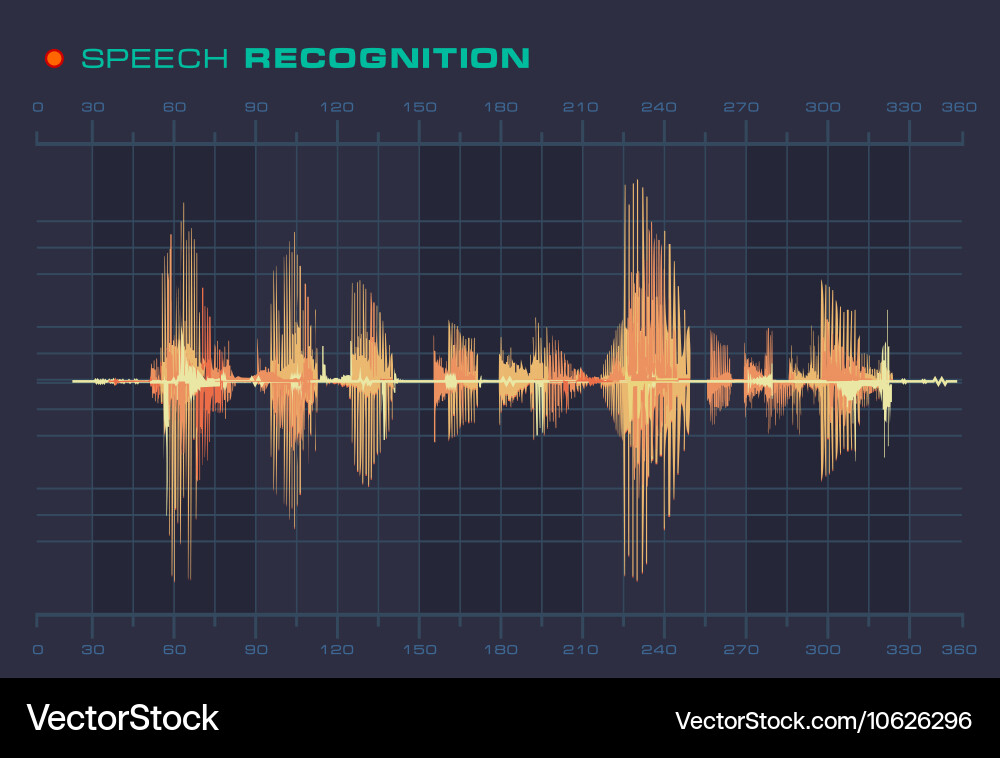
\includegraphics[width=0.6\linewidth]{org-download-images/introduction/2024-09-16_20-39-00_screenshot.png}
\caption{Image Courtesy: \href{https://cdn.vectorstock.com/i/1000v/62/96/speech-recognition-sound-wave-form-signal-diagram-vector-10626296.jpg}{[Stock Images on Web]​}}
\end{figure}
\end{frame}
\begin{frame}[label={sec:orgc2b43f6}]{spectral analysis}
\begin{itemize}
\item Waveform is a time series data.
\item Fourier Transform is a function that maps the
information in time domain to frequency domain.
\item Energy intensity histogram drawn against frequency
bands (or spectral bands), is called a spectrum.
\item Time domain information may be too dense to make
meaning of; hence frequency domain may be favoured.
\item Analysis in frequency domain is called spectral
analysis.
\end{itemize}
\end{frame}
\begin{frame}[label={sec:orge725335}]{spectrogram}
\begin{columns}
\begin{column}{.45\columnwidth}
\begin{figure}[htbp]
\centering
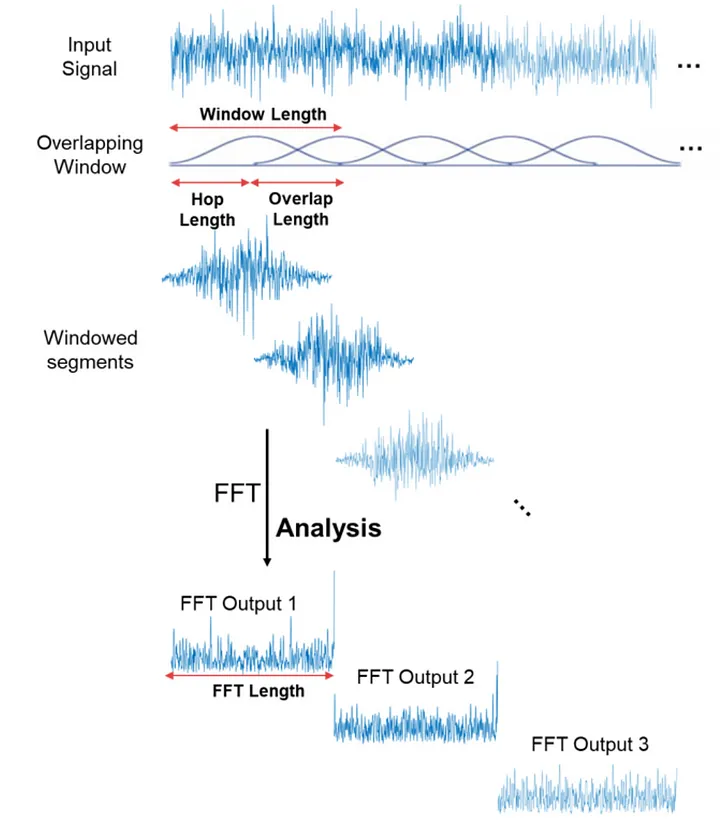
\includegraphics[width=.9\linewidth]{org-download-images/introduction/2024-09-16_20-59-46_screenshot.png}
\caption{Image Courtesy: \href{https://in.mathworks.com/help/dsp/ref/dsp.stft.html}{MathWorks}}
\end{figure}
\end{column}
\begin{column}{.55\columnwidth}
Spectrogram is a Short-Time Fourier Transform of the
input waveform; or “short-term power spectrum” of
sound.


\begin{figure}[htbp]
\centering
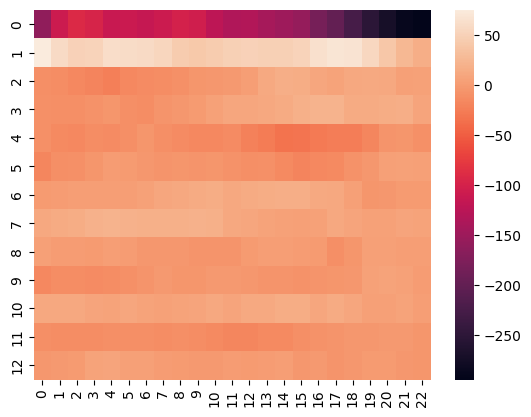
\includegraphics[width=0.75\linewidth]{org-download-images/introduction/2024-09-16_21-04-10_screenshot.png}
\caption{Spectrogram with 12 freq bands and 22 short-time windows.  Adapted from \href{https://colab.research.google.com/drive/1pkopM-0bSoxH1WDwq94bFSBxXpkHrjI3}{Lab 2: MFCC Example [Colab]​}.}
\end{figure}
\end{column}
\end{columns}
\end{frame}
\begin{frame}[label={sec:orgbf4059f}]{mel scale}
Mel (named after the word melody) is a non standard
perceptual scale of frequency, that is judged by
listeners to be equidistant from one-another.

\begin{figure}[htbp]
\centering
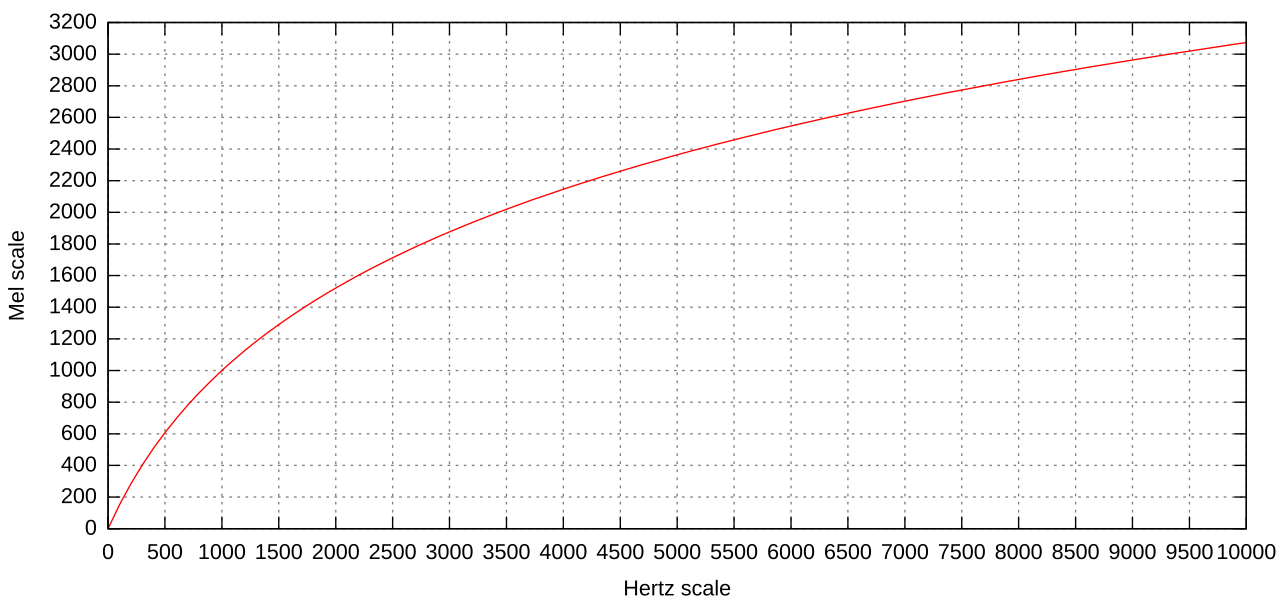
\includegraphics[width=0.75\linewidth]{org-download-images/introduction/2024-09-16_21-16-21_screenshot.png}
\caption{Image Courtesy: \href{https://en.wikipedia.org/wiki/File:Mel-Hz\_plot.svg}{[Wikimedia]​}}
\end{figure}
\end{frame}
\begin{frame}[label={sec:org2502c08}]{mel scale}
Mathematically, one of the linear+log fit looks like:
\begin{align*}
  m(f) &= \begin{cases}
    \frac{3f}{200}, &f<1000; \\
    15+27\log_{6.4}\left( \frac{f}{1000} \right),
                    &f\geqslant1000.
  \end{cases}
\end{align*}

This was popularised by \href{https://engineering.purdue.edu/\~malcolm/interval/1998-010/}{MATLAB Auditory Toolbox of
Slaney}
\end{frame}
\begin{frame}[label={sec:org26721fe}]{mel cepstrum}
Recall, that Spectrogram is a ``short-term power
spectrum.''

Mel-frequency cepstrum (MFC) is
\begin{itemize}
\item a short-term power spectrum,
\item based on linear cosine transform
\item of log-power-spectrum
\item on a non-linear mel scale of frequency.
\end{itemize}

Mel-frequency cepstral coefficients (MFCCs) are
coefficients that collectively make up an MFC.
\end{frame}
\begin{frame}[label={sec:orgf3af9b8}]{mfcc}
\href{https://medium.com/analytics-vidhya/understanding-the-mel-spectrogram-fca2afa2ce53}{Read More [Medium]​}
\end{frame}
\end{document}
